\documentclass[tikz,border=3pt]{standalone}
\usepackage{amsmath}
\usepackage[T1]{fontenc}
\usepackage[scaled=0.92]{helvet}
\renewcommand{\familydefault}{\sfdefault}
\usepackage{sansmath}
\usetikzlibrary{arrows.meta,positioning,fit,calc}
\begin{document}
\sffamily\sansmath\small
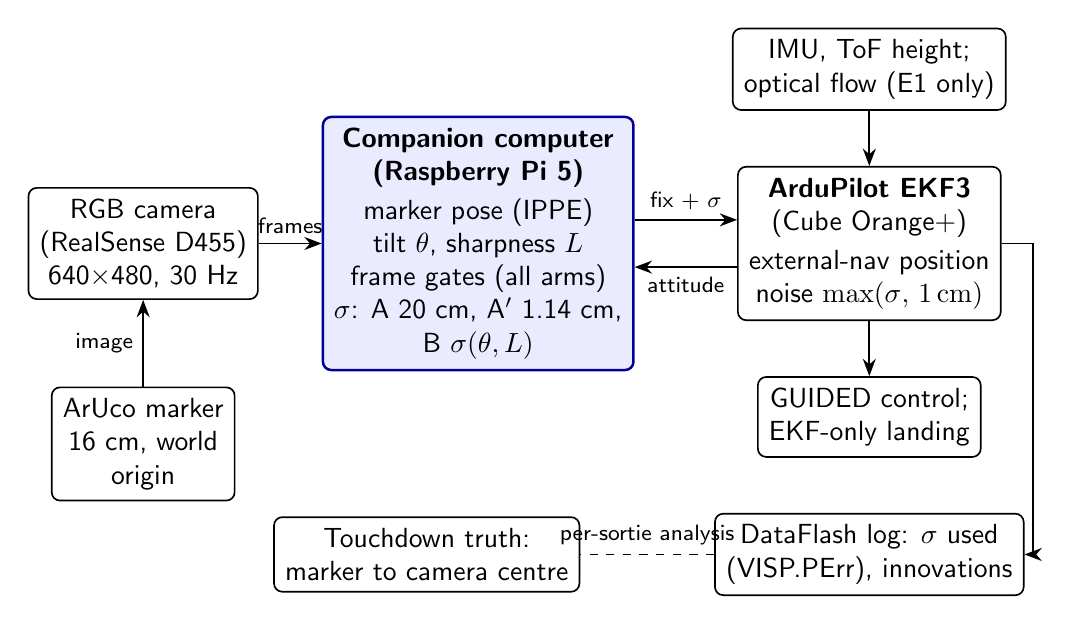
\begin{tikzpicture}[
  box/.style={draw,rounded corners=3pt,align=center,minimum height=9mm,inner sep=4pt,line width=0.6pt},
  hl/.style={box,fill=blue!8,draw=blue!60!black,line width=0.9pt},
  arr/.style={-{Stealth[length=2.2mm]},line width=0.6pt},
  dsh/.style={arr,dashed},
  lab/.style={font=\footnotesize,align=center}]
\node[box] (cam) {RGB camera\\(RealSense D455)\\640$\times$480, 30 Hz};
\node[box,below=11mm of cam] (marker) {ArUco marker\\16 cm, world\\origin};
\node[hl,right=8mm of cam] (pi) {\textbf{Companion computer}\\\textbf{(Raspberry Pi 5)}\\[2pt]
  marker pose (IPPE)\\tilt $\theta$, sharpness $L$\\frame gates (all arms)\\$\sigma$: A 20 cm, A$'$ 1.14 cm,\\B $\sigma(\theta,L)$};
\node[box,right=13mm of pi] (ekf) {\textbf{ArduPilot EKF3}\\(Cube Orange+)\\[2pt]external-nav position\\noise $\max(\sigma,\,1\,\mathrm{cm})$};
\node[box,above=7mm of ekf] (sens) {IMU, ToF height;\\optical flow (E1 only)};
\node[box,below=7mm of ekf] (ctl) {GUIDED control;\\EKF-only landing};
\node[box,below=7mm of ctl] (log) {DataFlash log: $\sigma$ used\\(VISP.PErr), innovations};
\node[box,left=17mm of log] (truth) {Touchdown truth:\\marker to camera centre};
\draw[arr] (marker) -- node[lab,left]{image} (cam);
\draw[arr] (cam) -- node[lab,above]{frames} (pi);
\draw[arr] ($(pi.east)+(0,3mm)$) -- node[lab,above]{fix + $\sigma$} ($(ekf.west)+(0,3mm)$);
\draw[arr] ($(ekf.west)+(0,-3mm)$) -- node[lab,below]{attitude} ($(pi.east)+(0,-3mm)$);
\draw[arr] (sens) -- (ekf);
\draw[arr] (ekf) -- (ctl);
\draw[arr] (ekf.east) -- ++(4mm,0) |- (log.east);
\draw[dashed,line width=0.6pt] (log.west) -- node[lab,above]{per-sortie analysis} (truth.east);
\end{tikzpicture}
\end{document}
